\documentclass[12pt]{article}

\usepackage[figures]{uproject}
\usepackage[utf8]{inputenc}
\usepackage{epsfig}

\title{Projektový seminář}
\subtitle{Latrunculi}
\author{Ondřej Grätz}
\group{Aplikovaná informatika, III. ročník}
\date{Červen 2016}

\docinfo{Ondrej Gratz}{Latrunculi}

\abstract{Implementace deskové hry Latrunculi s~použitím \emph{.NET Framework} pro~operační systém \emph{Windows}.}

\begin{document}
\maketitle

\newpage
\section{Zadání projektu}
Cílem projektu je vytvoření hry pro desktopový operační systém s~grafickým uživatelským rozhraním (GUI) dle standardů.

Požadavek na přenositelnost spustitelných souborů nebyl stanoven. Uživatelské rozhraní se~předpokládá objektově orientované s~použitím oken a~standardních prvků (hlavní nabídka, nástrojová lišta, tlačítka).

\section{Volba technologie}
\subsection{Výběr operačního systému}
Já jsem pro vývoj i~běh hry (aplikace) zvolil operační systém \emph{Windows}, jelikož je~mi~dobře známý a~také proto, že je to s~podílem 52~\% (viz~\cite{wiki2016}) mezi uživateli i programátory nejpoužívanější operační systém pro osobní počítače.

\subsection{Výběr vývojového prostředí}
Pro vývoj byl zvolen nástroj \emph{Visual Studio} od firmy \emph{Microsoft}, jazyky \emph{C\#} a~\emph{F\#} a~pro vývoj uživatelského rozhraní \emph{Windows Presentation Framework} (WPF).

Pro zvolený operační systém (\emph{Windows}) by~s~ohledem na~zadání bylo výhodné použít jeden z~následujících typů aplikací. 
	\begin{itemize}  
		\item Win32 (Visual C++ s použitím Windows API nebo MFC)
		\item .NET Framework + WinForms
		\item .NET Framework + WPF
		\item Windows Runtime (C++/CX) 
	\end{itemize}

\emph{Win32} a \emph{Windows Runtime} poskytují nejmenší úroveň abstrakce. Vývoj tohoto typu aplikací vyžaduje větší znalosti a~zkušenosti programátora. \emph{Windows Runtime} aplikace je navíc možné spustit pouze pod~operačním systémem \emph{Windows~8} (nebo novějším). Výhodou je ale standardní vzhled výsledných aplikací a~nejlepší výpočetní výkon.

Použití \emph{WinForms} by bylo výhodné, jelikož vývoj je jednoduchý (údálostmi řízený, objektově orientovaný). Výsledná aplikace má~vzhled v~souladu se~standardy operačního systému a~očekáváním uživatele. Nevýhodou je~strohý design, který se~příliš nepřizpůsobuje rozlišení obrazovky a~jehož vzhled se~může jevit zastaralý. Design je~navíc velmi svázán s~kódem, který má~na~starosti výpočty a~samotnou logiku aplikace.

Naproti tomu u~\emph{WPF} je již při vývoji myšleno na responzivní design. Prvky uživatelského rozhraní mají velmi bohaté a~pro programátora snadno použitelné vlastnosti, které umožňují přízpůsobit aplikaci různým velikostem obrazovky a~různým způsobům vstupu od uživatele (dotykové obrazovky, přizpůsobení pro zrakově nebo tělesně hendikepované uživatele). Návrh uživatelského rozhraní je~navíc velmi dobře oddělen od samotného kódu a~umožňuje s~použitím nástroje \emph{Microsoft Blend} výrazně zasáhnout do designu aplikace i~grafikovi (bez nutnosti znalosti programování a~bez zásahu do~modelu aplikace).

\section{Organizace kódu}
\subsection{Zvyklosti pro .NET aplikace}
Při vývoji pro \emph{.NET Framework} je nutno veškerý kód umisťovat do metod tříd. Třídy musejí být povinně organizovány do jmenných prostorů. Jmenné prostory je~vhodné stromově strukturovat dle~navržené architektury aplikace.

Pro \emph{.NET} aplikace (s výjimkou aplikací v jazyku F\#) je~typické rozdělení zdrojového kódu do~několika projektů, které jsou přidány do~skupiny projektů (Solution). Rozdělení se~provádí na~základě jmenných prostorů (\texttt{namespaces}) tak, aby třídy patřící do stejného prostoru byly ve~stejném projektu. 

Spustitelný (EXE) soubor obsahje jádro programu a~definice hlavních částí uživatelského rozhraní, ale komponenty uživatelského rozhraní i~třídy obsahující doménový nebo datový model, rozhodovací logiku a~třídy pro práci se soubory, databázemi či~síťovou komunikaci jsou umístěny v~tzv.~knihovnách tříd (DLL soubory). Toto dělení poté představuje výhodu při požadavku na~změnu typu výsledné aplikace. Lze například textové rozhraní aplikace nahradit GUI. Nebo nahradit samostatně spustitelnou konzolovou aplikaci službou systému Windows. Společné součásti tak mohou být opětovně využívány (sdíleny).

DLL~i~EXE soubory poté obsahují překladačem vytvořený \emph{bytecode}, který je~poté při spuštění aplikace částečně kompilován do strojového kódu (just-in-time kompilace) a~částečně také interpretován běhovým prostředím \emph{.NET}.

\subsection{Prevence cyklických závislostí}
Abstraktní rozdělení kódu na vrstvy pomáhá při vývoji předcházet cyklickým (rekurzivním) závislostem mezi třídami (respektive mezi jednotlivými knihovnami tříd). Nevhodné závislosti mezi třídami by~totiž mohly při dokončování aplikace způsobit komplikace, které by~v~krajním případě bránily překladu aplikace a~vyžadovaly by~refaktorování celého kódu. Jako prevence se~proto činnosti jednotlivých součástí seskupují tak, aby vyšší vrstvy byly závislé na nižších vrstvách. Nevhodné je naopak odkazovat se~z~nižších vrstev na~vyšší, ačkoliv i~tato možnost může být potřebná. V~případě potřeby se~ale namísto reference používají události tak, že nižší vrstva generuje událost a~vyšší vrstva událost zachytává. Bližší informace viz~\cite{wlaschin1}.

\subsection{Soubory projektu}
Třídy projektu jsou organizovány v~podprostorech jmenného prostoru \texttt{Latrunculi}. 

Rozvrstvení aplikace je~zobrazeno na~obr.\ref{Layers}. Tomu odpovídající výsledné přeložené soubory (assemblies) a~jejich závislosti jsou zobrazeny na~obr.\ref{Assemblies}. Názvy souborů jsou shodné s~názvy jmenných prostorů, které jsou v~jednotlivých souborech obsaženy. Výjimku tvoří spustitelné soubory, u~kterých je záměrně oproti názvu jmenného prostoru, který obsahují, vynechána tečka, aby bylo případné spouštění z~příkazového řádku pohodlnější.

\begin{figure}[ht]
  \centering
  \begin{minipage}[b]{0.4\textwidth}
		\center{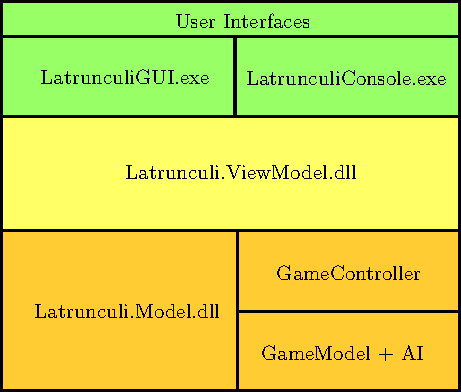
\includegraphics[height=60mm]{Layers.pdf}}
		\caption{Vrstvy aplikace}
		\label{Layers}
  \end{minipage}
  \hfill
  \begin{minipage}[b]{0.4\textwidth}
		\epsfysize=70mm
		\center{\epsfbox{Assemblies.eps}}
		\caption{Závislosti souborů}
		\label{Assemblies}
  \end{minipage}
\end{figure}

\section{Rozvrstvení aplikace}
\subsection{Vrstva uživatelského rozhraní}
Nejvyšší vrstvou v našem diagramu z~obr.\ref{Layers} je \emph{User Interface}, tj. uživatelské rozhraní. Vrstva je~horizontálně rozdělena, jelikož naše aplikace má dva typy uživatelských rozhraní. Konzolové rozhraní (\texttt{Latrunculi.ConsoleUI}) a~grafické rozhraní (\texttt{Latrunculi.GUI}).


\begin{figure}[ht]
	\epsfysize=200mm
	\center{\epsfbox{PrimaryUseCases.eps}}
	\caption{Případy užití}
	\label{PrimaryUseCases}
\end{figure}

\newpage
\begin{thebibliography}{10}
	
\bibitem{outr2008} Mgr. Jan Outrata, Ph.D.: \emph{Projekt - implementace},
 \url{http://outrata.inf.upol.cz/courses/ps/navrh.pdf},
			listopad~2008.

	
\bibitem{outr2010} Mgr. Jan Outrata, Ph.D.: \emph{Projekt - analýza a návrh},
 \url{http://outrata.inf.upol.cz/courses/ps/implementace.txt},
			listopad~2010.

\bibitem{kuhr2011} Mgr. Tomáš Kühr, Ph.D.: \emph{Algoritmy realizující počítačového hráče},
 \url{http://www.inf.upol.cz/downloads/studium/PS/algoritmy.pdf},
			říjen~2011.

\bibitem{wiki2016}Wikipedia: \emph{Usage share of operating systems},
 \url{https://en.wikipedia.org/wiki/Usage_share_of_operating_systems#Desktop_and_laptop_computers},
			květen~2016.

\bibitem{wlaschin}Scott Wlaschin: \emph{F\# For Profit And Fun},
 \url{https://fsharpforfunandprofit.com/},
			květen~2016.

\bibitem{wlaschin1}Scott Wlaschin: \emph{Dependency Cycles},
 \url{https://fsharpforfunandprofit.com/series/dependency-cycles.html},
			květen~2016.


\end{thebibliography} 

\end{document}
